\documentclass[Ex4_Zusammenfassung.tex]{subfiles}


\begin{document}
	
\chapter{Einleitung - Ex3 Zusammenfassung}
Wir hatten die QUANTENMECHANIK eingeführt, siehe Theo 4:\\

$ \fbox{\parbox{\dimexpr\linewidth-2\fboxsep-2\fboxrule\relax}
	{\centering 
		\textbf{Axiom 4:  Es gilt die  Schrödingergleichung: \ } 
		$  \hat{H} \ket{\psi} = i \hslash \partial_t \ket{\psi}\ $ \\
		wobei $ \hat{H} := \frac{\hat{p}^2}{2m} + \hat{V} = - \frac{\hslash^2}{2m} \nabla^2 + V$
		 } } $ \\

Diese hatten wir für das Wasserstoffatom (H-At.) \textbf{analytisch} gelöst. (Coulombpotential, Kugelkoordinaten, Separation: Schwerpunkt/Relativbew., Winkel-/Radialanteil). Die Lösungen sind Polynome mit ganzzahligen Parametern, "Quantenzahlen":
\begin{align*}
	\psi_{n,l,m_l}\lp r, \vartheta, \varphi \rp &= R_{n,l} (r) \cdot \Theta_l^{m_l} (\vartheta) \cdot \phi_{m_l} (\varphi)\\
	\psi_{n,l,m_l} &\propto\  \mathrm{e}^{- \frac{Zr}{na_0}}\  \underbrace{L_{n-l-1}^{2l+1} \lp \frac{2Zr}{na_0} \rp \cdot P_l^{m_l} (\cos{\vartheta})}_{\mathclap{\text{zugeordnete Laguerre- bzw. Legendrepolynome.}}} \cdot \frac{1}{\sqrt{2\pi}} \mathrm{e}^{im_l \varphi}\\
\end{align*}

Es gilt für physikalische Lösungen: $\boxed{ | m_l | \leq l < n } $\\ 

\section{Notation der Quantenzahlen}
Hauptquantenzahlen $n\ \in \{ 1, 2, 3, ... \} = \{K, L, M, ...\}$ ''Schale'' \\
Bahndrehimpulsquantenzahlen $ l \in \{0, 1, 2, ...\} = \{s, p, d, f, ...\} $ ''Unterschale'' \\
Magnetbahnquantenzahlen $m_l \in \{-l, -l+1, ... , l \}$ ''Orbital'' (zzgl. ''Spin'')\\
\begin{equation*}
	E \lp \psi_n \rp = E_n = -E_0 \frac{Z^2}{n^2}
\end{equation*}
''Rydberg-Formel'', mit $E_0 := Ry =\SI{13.6}{\eV} $ und $Z$ als Kernladungszahl.\\
Dem Übergang entspricht dann die Differenz $E_n - E_m$.

\section{Korrekturterme der Energieniveaus}
Die Energieniveaus (EN) werden korrigiert durch:
\begin{align*}
	\hat{H} &= \hat{H}_0 + \underbrace{ \Delta \hat{E}_{\text{rel}} + \Delta \hat{E}_{S-B} + \Delta \hat{E}_{\text{Darwin}} }_{\mathclap{\sum\ = \text{ Feinstruktur } \Delta E_{FS}} } + \Delta \hat{E}_{\text{Lamb}} + \Delta \hat{E}_{\text{HFS}} + \Delta \hat{E}_{\text{Zeeman}}\\
	\hat{H}_0 &= \frac{\hat{p}^2}{2m_e} + \hat{V}\\
	\Delta \hat{E}_{\text{rel}} &= - \frac{p^4}{8 m_e^3 c^2} \\
	& \kern -3.1em \begin{rcases}
		\Delta \hat{E}_{\text{S-B}} = \frac{Z q_e^2 \mu_0}{8 \pi m_e^2 \braket{r}^3}\ \hat{\vec{l}} \cdot \hat{\vec{s}} = \frac{Z q_e^2 \mu_0 \hslash^2}{16 \pi m_e^2 \braket{r}^3} \cdot 
			\begin{cases}
				l,&  j=l+\frac{1}{2}\\
				-(l+1) ,& j=l-\frac{1}{2}
			\end{cases} \\
	\kern -1.3em \Delta \hat{E}_{\text{Darwin}} = \mu_0 \lp \frac{q_e \hslash}{m_e} \rp^2 Z \cdot \delta\lp \vec{r} \rp\  \text{''Kernpotential''} 
	\end{rcases}
	\Delta \hat{E}_{FS} \stackrel{\mathclap{\text{\tiny{H-At.}}}}{=} E_0 \frac{Z^2}{n^2} \left[ \frac{Z^2 \alpha^2}{n} \lp \frac{1}{j+\frac{1}{2}} - \frac{3}{4n} \rp  \right] \\
	& \kern -3.55em \Delta \hat{E}_{\text{Lamb}}\  \widehat{=} \text{ quantenelektrodynamische Wechselwirkung (WW) mit dem Vakuum}\\
	& \kern -3.1em \Delta \hat{E}_{\text{HFS}} \propto\ \vec{J} \cdot \underbrace{\vec{I}}_{\mathclap{\text{''Kernspin''}}}\\
	& \kern -4.2em \Delta \hat{E}_{\text{Zeeman}} = \frac{\mu}{\hslash} \lp \hat{L}_z + g_e \hat{S}_z \rp B_z\ \text{''anomal'', normal für } \hat{S}_z = 0\ ,\ g_e \approx 2\ ,\ \mu = \frac{q_e \hslash}{2m_e}
\end{align*}

\section{Näherungen für mehrere Elektronen}
Für mehrere Elektronen $ \lp e^- \rp $ müssen wir Näherungen machen, denn die $ e^- - e^- - WW$ verhindert das analytische Lösen. \\

\textbf{Helium (He):}
\begin{enumerate}
	\item $E_B = - Z^2 E_0 \lp \frac{1}{n_1^2} + \frac{1}{n_2^2} \rp \ \text{''Bindungsenergie'' (negativ!)}$
	\item $E_B = - E_0 \lp \frac{Z^2}{1^2} + \frac{(Z-1)^2}{n_2^2} \rp\ \text{Abschirmung des } n_2-e^-$
	\item $E_B = -E_0 \lp-2Z_R^2 + (4Z - \frac{5}{4}) Z_R \rp\ \text{minimiere } E_B(Z_R) $
	\item wahrer Wert $ E_B \approx \SI{-79.0}{\eV}$
\end{enumerate}

\section{Das Pauli-Prinzip}
Die relativistische Quantenmechanik fordert für Teilchen mit Spin $\frac{1}{2},\ \frac{3}{2},\ ... $ [ bzw. 0, 1, 2, ... ] eine unter Teilchenvertauschung $\hat{P}_{ij} $ antisymmetrische [bzw, symmetrische] \textbf{Gesamtwellenfunktion} $ \ket{\psi} = \ket{\psi_{\text{Ort}}} \otimes \ket{\chi_{\text{Spin}}} $. Wir nennen diese Teilchen \textbf{Fermionen} [bzw. \textbf{Bosonen}]. Aus diesem Postulat folgt das:\\


\fbox{\parbox{\dimexpr\linewidth-2\fboxsep-2\fboxrule\relax}
	{\centering 
		\textbf{Paul\tiny{i}\small{-Prinzip:} \ } Man kann nie mehr als ein Fermion im gleichen (Orts- \& Spin-) Zustand haben.} }\\

Für zwei $e^-$ (z.B. Helium) gilt daher:
\begin{align*}
	\ket{\psi_{\text{Ort}}}_{\text{symm.}} &\Rightarrow \underbrace{\ket{\chi_-}}_{\mathclap{\text{Dies ist ein \textbf{anti}symmetrisches Singulett [2S+1=1] }}} = \frac{1}{\sqrt{2}} \lp \ket{\uparrow_1\ \downarrow_2} - \ket{\downarrow_1\ \uparrow_2} \rp\  \widehat{=} \underbrace{\ket{S=0, M_S=0}}_{\mathclap{\substack{\text{ [Großbuchstaben } S,\ M_S,\ J,\ ... \\ \text{ sind Gesamtquantenzahlen, Summen] } }} }\\
	& \kern -5.95em \begin{rcases}
		\ket{\psi_{\text{Ort}}}_{\text{antisym.}} \Rightarrow &\ket{\chi_+ ,\ 1} = \ket{\uparrow_1\ \uparrow_2} \\
		&\ket{\chi_+ ,\ 0} = \frac{1}{\sqrt{2}} \lp \ket{\uparrow_1\ \downarrow_2} + \ket{\downarrow_1\ \uparrow_2} \rp\\
		&\ket{\chi_+ ,\ -1} = \ket{\downarrow_1\ \downarrow_2}
	\end{rcases} 
	\widehat{=} 
		\begin{array}{l}
			\ket{S=1,\ M_S=0}\\
			\ket{1,\ 0}\\
			\ket{1,\ -1}
		\end{array}
\end{align*}

$\ket{\chi_+,\ -}$ ist ein \textbf{symm}etrisches Triplett [2S+1=3 heißt Multiplizität].

\chapter{ Ex4 - 1.Vorlesung und Einführung}

In der Ex4-Vorlesung wird es um folgende Themen gehen:

\begin{itemize}
\item Atome
\item Kerne und Elementarteilchen
\item Symmetrien
\item schwache und starke Wechselwirkung
\item Spaltung und Fusion 
\end{itemize}
Johanna Stachels Notation: 
\begin{align*}
& e^2 = \frac{q_e^2}{4\pi \epsilon_{0}}  \\
%%
& 1 \ eV = 1.60 \cdot 10^{-19} J  \\
& 1 \ fm = 913 \ \nicefrac{MeV}{c^2} = 1.66 \cdot 10^{-27} kg \\
& \hslash = 6.58 \cdot 10^{-16} eVs = 1.05 \cdot 10^{-34} Js \\
&\alpha = \frac {e^2}{c \hslash} = \frac{1}{137} \\
&c = 3 \cdot 10^8 \  \nicefrac{m}{s} \\
\end{align*}

\section{Spektroskopische Notation}
Um den Zustand einer Unterschale nl anzugeben, führen wir die spektroskopische Notation ein: 
\begin{equation}
\centering \boxed{ n \ ^{2S+1}L_J }
\end{equation}
mit
\begin{align*}
&S := | \sum_{i} m_{s,i}\ \quad |L:=  | \sum_{i} m_{l,i} | \\
&J := \left| \vec L + \vec S \right|  = | M_L + M_S |   = | \sum_{i} m_{l,i} + \sum_{i} m_{s,i}  | 
\end{align*}
\newline
Die Notation für die Elemente des Periodensystems lautet: 
\begin{equation}
\centering \boxed{^{\qquad Massenzahl \  \frac{m}{u} } _{Kernladungszahl \  Z} \  El ^{\ \frac{q}{q_e} \  Ionisierung}} 
\end{equation}

\section{Hund'sche Regeln und Auswahlregeln}
Die Elektronen werden für die Grundzustände so aufgefüllt, dass die Bindungsenergie(negativ) minimiert wird, das heißt deren Betrag maximal wird. Zwischen den Unterschalen gilt folgende Reihenfolge: \\ \newline
	\begin{figure}[h]
	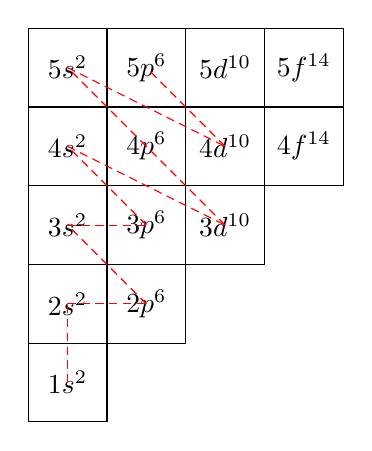
\begin{tikzpicture}
	\draw (0,0) +(-.5,-.5) rectangle ++(.5,.5);
	\draw (0,0) node{$1s^2$};
	\draw (0,1) +(-.5,-.5) rectangle ++(.5,.5);
	\draw (0,1) node{$2s^2$};
	\draw (0,2) +(-.5,-.5) rectangle ++(.5,.5);
	\draw (0,2) node{$3s^2$};
	\draw (0,3) +(-.5,-.5) rectangle ++(.5,.5);
	\draw (0,3) node{$4s^2$};
	\draw (0,4) +(-.5,-.5) rectangle ++(.5,.5);
	\draw (0,4) node{$5s^2$};

	\draw (1,1) +(-.5,-.5) rectangle ++(.5,.5);
	\draw (1,1) node{$2p^6$};
	\draw (1,2) +(-.5,-.5) rectangle ++(.5,.5);
	\draw (1,2) node{$3p^6$};
	\draw (1,3) +(-.5,-.5) rectangle ++(.5,.5);
	\draw (1,3) node{$4p^6$};
	\draw (1,4) +(-.5,-.5) rectangle ++(.5,.5);
	\draw (1,4) node{$5p^6$};

	\draw (2,2) +(-.5,-.5) rectangle ++(.5,.5);
	\draw (2,2) node{$3d^{10}$};
	\draw (2,3) +(-.5,-.5) rectangle ++(.5,.5);
	\draw (2,3) node{$4d^{10}$};
	\draw (2,4) +(-.5,-.5) rectangle ++(.5,.5);
	\draw (2,4) node{$5d^{10}$};

	\draw (3,3) +(-.5,-.5) rectangle ++(.5,.5);
	\draw (3,3) node{$4f^{14}$};
	\draw (3,4) +(-.5,-.5) rectangle ++(.5,.5);
	\draw (3,4) node{$5f^{14}$};

	\draw [draw = red, densely dashed] (0,0) -- (0,1);
	\draw [draw = red, densely dashed] (0,1) -- (1,1);
	\draw [draw = red, densely dashed] (1,1) -- (0,2);
	\draw [draw = red, densely dashed] (0,2) -- (1,2);
	\draw [draw = red, densely dashed] (1,2) -- (0,3);
	\draw [draw = red, densely dashed] (0,3) -- (2,2);
	\draw [draw = red, densely dashed] (2,2) -- (1,3);
	\draw [draw = red, densely dashed] (1,3) -- (0,4);
	\draw [draw = red, densely dashed] (0,4) -- (2,3);
	\draw [draw = red, densely dashed] (2,3) -- (1,4);
	\end{tikzpicture}
	\caption{Auffüllung der Grundzustände}
	\end{figure}
	\\ \newline
	Pro Unterzustand hat man $ N_e = 2(2l+1) $ Elektronen. 
	Die Gesamtzahl der Elektronen in der n-ten Schale entspricht somit $ N_e = 2 \sum_{l}^{n-1} 2l+1 =   2n^2 $

Innerhalb einer Unterschale gelten für die Grundzustände die hierarchischen \textbf{Hund'schen Regeln}: 
\begin{enumerate}
\item Wenn $  | \sum_{i} m_{s,i} | \text{ maximal } \Rightarrow $ S maximal und $ S =  | \sum_{i} m_{s,i} |$. 
\item Wenn $  | \sum_{i} m_{l,i} | \text{ maximal } \Rightarrow $ L maximal und $ L =  | \sum_{i} m_{l,i} |$. 
\item Ist die Unterschale bis zu (einschließlich) halb voll, so wird J minimal d.h \\  $ J \stackrel{!}{=} \lvert L-S \rvert $ , bei mehr als halb vollen Unterschalden muss $ J \stackrel{!}{=} | L+S | $ sein. 
\end{enumerate} 

Diese Regeln bestimmen die Feinstruktur des Elements. Regt man das Element an, so gelten diese Regeln nicht mehr.  \newpage Die Schalen-/Orbitalübergänge werden von den sog. \textbf{Auswahlregeln} beherrscht, die wohlgemerkt nicht hierarchisch sind. 
\begin{enumerate}
\item $ \Delta L \  \in $ \{-1,1\}  bei L-S-Kopplung
\item $ \Delta M_L \   \in  $ \{-1,0,1\}  
\item $ \Delta S =0 $ für leichte Atome
\item $\Delta J \  \in $  \{-1,0,1\}   wobei $ \ J =0 \  \rightarrow J=0 \  \textbf{verboten} $
\end{enumerate}

\section{Vielelektronenprobleme} 
Für Elemente mit mehr als einem Elektron gibt es keine analytische Lösung der Schrödinger-Gleichung, auch numerische Verfahren sind mit zunehmender Elektronenzahl extrem aufwändig. Wir machen deshalb folgende Näherungen:
\textbf{Alkaliatome (1.Hauptgruppe)} \newline 
\begin{itemize}
\item Alkaliatome haben nur ein Elektron außerhalb geschlossener Schalen. Die Grundzustände sind immer $ \ ^{2}S_{\frac{1}{2}} $ ( $ n  \in \{2,3,4,...\} $ nicht notiert).
\item Wir betrachten zu Näherung ein \textbf{effektives Potential} $ V_{eff}(r) $ \newline \newline
 $ V_{eff}(r) = - \frac{e^2 Z_{eff}(r)}{r} $ mit $ 1 < Z_{eff}(r) < Z $ \  und  $ Z_ {eff} \stackrel{r\rightarrow \infty}{\rightarrow} 1, \ Z_{eff} \stackrel{r \rightarrow 0}{\rightarrow} Z $
 
\begin{figure}[h]
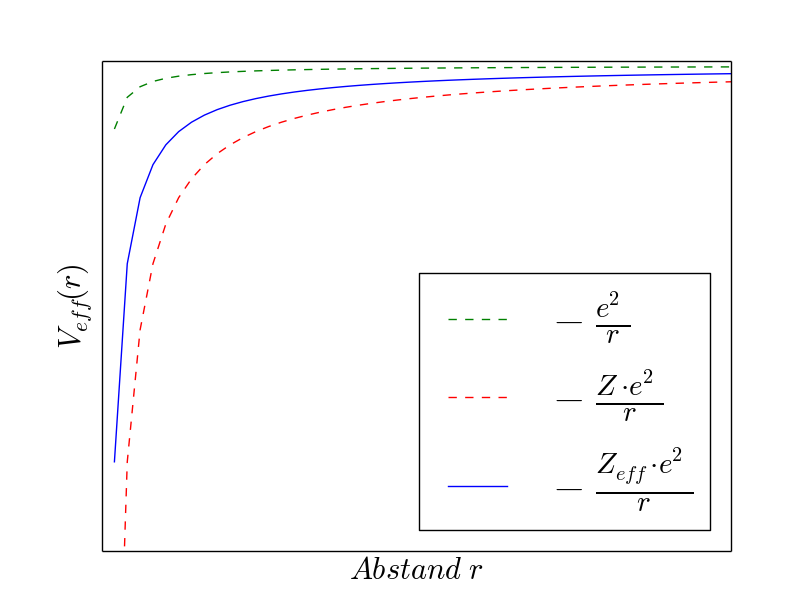
\includegraphics[height= 6cm, width=9cm]{effpot.png}
\caption{ Effektives Potential }
\end{figure}
 \item Dies hebt die $ E_n $ -Entartung bezüglich Z bereits auf (Feinstruktur): \newline
$ E_n(s) < E_n(p) < E_n(d) < E_n(f)$ (für kleine n am stärksten)
\item Für große n und r (wasserstoffähnlich) lässt sich dies so schreiben: 
 	\begin{equation}
 	E_{n,l} = -E_0 \frac{Z_{eff}^2}{n^2} = - \frac{E_0}{n_{eff}^2} = - \frac{E_0}{(n-\delta_{n,l})^2} 			\qquad E_0 = 13.6 \  eV 
 	\end{equation}
 wobei $\delta_{n,l} $ der sog. \textbf{Quantendefekt} ist: $ \delta_{n,l} = n - \sqrt{\frac{E_0}{-E_{n,l}}} \newline  E_{n,l} <\  0  $ ist die real gemessene Energie. 

\end{itemize}
Um allgemeine Vielelektronenprobleme zu lösen, können wir (zumindest bis jetzt) nur nähern indem wir zur Lösung eines Elektron die anderen Elektronen unabhängig voneinander gelöst habe und das entstehen $ V_{eff}(r) $ \textbf{kugelsymmetrisch} ist. \newline
Wir suchen deshalb eine  \textbf{Gesamtwellenfunktion für N Teilchen}. \newline
Diese muss antisymmetrische unter Vertauschung sein, wir nehmen zusätzlich an, dass sie sich als Produkt der Einteilchenwellenfunktionen schreiben lässt. \newline 
Analog zu $ \psi_{ges}(1,2) = \psi_1(1) \psi_2(2) - \psi_2(1) \psi_1(2) $  definieren wir die \\ \textbf{Slaterdeterminante}: 
	\begin{equation}
	  \psi_{ges}(r_1,...,r_N) \ = \  \frac{1}{\sqrt{N!}} \  det \begin{pmatrix} \psi_1(1) & \psi_1(2) & \dots & \psi_1(N) \\ \vdots & \vdots & \vdots & \vdots \\  \psi_N(1) & \psi_N(2) & \dots & \psi_N(N)  \end{pmatrix} 
	\end{equation}
Diese ist total antisymmetrisch unter Spaltenvertauschung als Summe aus N! Produkten. 
\section{Moseley-Gesetz}
Für Eletronen-übergänge zwischen Zuständen wurde empirisch festgestellt, dass $ \sqrt{f} \propto Z $ ist, wobei f die Frequenz des emittiereten Lichts ist. 
\begin{align*}
\textbf{Moseley Gesetz:} \ f \ &= \ E_0 c (\nicefrac{1}{n_2^2} - \nicefrac{1}{n_1^2}) \ (Z-b)^2 \\ 
mit \  c \  = \    \lambda f \ :   \	\lambda \ & = \ E_0 (\nicefrac{1}{n_2^2} - \nicefrac{1}{n_1^2}) \ (Z-b)^2
\end{align*}
für Übergänge $ n_1 \rightarrow n_2 $ , b - Abschirmkonstante \newline
Für das Wasserstoffatom entspricht das Moseley-Gesetz der Rydberg-Formel. \newline
Für wasserstoffähnliche Atome (b=1) gilt : \quad K-Linie: $ n_2 = 1, \  \alpha :  n_1 = 2, \  \beta: n_1 = 3 $ \newline
Für schwere Atome ($ Z > 40 $  )  gilt :  \qquad L-Linie: $ n_2 = 2 , b \approx 7.4 , \ \alpha : \ n_1= 3 , \  \beta: n_1 = 4 $ \newline
Die Auswahlregeln müssen gelten. 

\end{document}
 

